%==============================================================================
\section{Como instalar?}
%==============================================================================
%
\begin{citacao}
\textbf{Atenção:} esse texto considerará sistemas \textit{Windows}, 
\unit[64]{bits}, cuja distribuição de \LaTeX\ seja o MiK\TeX.
Logo, caso seu sistema ou distribuição sejam diferentes, adaptações 
provavelmente serão necessárias.
\end{citacao}
 
Na pasta intitulada \texttt{classe\_ativmatUFRB}, existem arquivos e subpastas.
Daremos, a seguir, uma sucinta explanação sobre cada um deles:

\begin{itemize}
  \item \textbf{figs} É uma pasta que contém o logotipo\footnote{há também 
   outra figura que foi usada como exemplo na lista.
   Tal figura, pode ser descartada depois.} da \textsc{ufrb} utilizado no 
   cabeçalho (que não deve ser deletado).
   Caso sua lista de atividade contenha figuras, estas devem ser colocadas 
   exclusivamente nesta pasta.
  \item \textbf{fonts} Contém arquivos de extensão \texttt{.ttf} da fonte
   \href{https://www.tug.org/FontCatalogue/intimacy/}{intimacy}.
   \marginpar{\qrcode[height = 1cm]{https://www.tug.org/FontCatalogue/intimacy/}}
  \item \textbf{ativmatUFRB.cls} A classe em si, ou seja, o conjunto de 
   modificações que implementam as necessidades básicas de uma lista de 
   atividade com cabeçalho estilizado para um curso de Matemática da \textsc{ufrb}. 
  \item \textbf{modelo\_ativmatUFRB.pdf} Resultado final, de extensão 
   \texttt{.pdf}, produzido ao compilar o modelo em questão.
  \item \textbf{modelo\_ativmatUFRB.tex} Modelo de Lista de Atividade que
   explora os comandos internos da classe. 
   Nesse arquivo também há comentários (marcados com ``\%'') para auxilio dos 
   usuários.
  \item \textbf{README.md} Texto com explicações gerais sobre a classe, 
   geralmente usado em repositórios (como o \href{https://github.com/}{GitHub}).
   \marginpar{\qrcode[height = 1cm]{https://github.com/}}
\end{itemize}

Uma estruturação visual é pode ser vista a seguir:

\begin{codbox}{Árvore de Diretórios da pasta}
 \begin{forest}
  pic dir tree,
  pic root,
  for tree={directory,},
  [classe\_ativmatUFRB
   [figs
     [espiral.pdf, file]
     [ufrb.jpeg, file]
   ]
   [fonts
     [intimacy
       [intimacy.ttf, file]
       [intimcy2.ttf, file]
     ]
   ]
   [ativmatUFRB.cls, file]
   [modelo\_ativmatUFRB.pdf, file]
   [modelo\_ativmatUFRB.tex, file]
   [README.md, file]
  ]
 \end{forest}
\end{codbox}

Basicamente, para você obter o resultado da classe \texttt{ativmatUFRB} para 
uma lista de atividade de sua autoria, deverá ter:

\begin{itemize}
  \item Se você ainda usa \texttt{pdfLaTeX}:
   \begin{itemize}
	   \item A classe \texttt{ativmatUFRB.cls};
    \item O arquivo \texttt{modelo\_ativmatUFRB.tex};
    \item Uma pasta com o nome \texttt{figs}, que deve conter o arquivo. 
     \texttt{ufrb.jpeg}
   \end{itemize}
  \item Se você usa \texttt{LuaLaTeX} ou \texttt{XeLaTeX} (recomendados):
   \begin{itemize}
    \item A classe \texttt{ativmatUFRB.cls};
    \item O arquivo \texttt{modelo\_ativmatUFRB.tex};
    \item Uma pasta com o nome \texttt{figs}, que deve conter o arquivo 
     \texttt{ufrb.jpeg}; 
    \item E a pasta \texttt{fonts} com os arquivos da fonte \texttt{intimacy}.
   \end{itemize}
\end{itemize}

\begin{citacao}
  É aconselhável não modificar o arquivo \texttt{ativmatUFRB.cls}. 
\end{citacao}

Por isso, é importante armazená-lo em local apropriado.
Uma boa prática, para organização pessoal, é salvar cada atividade em uma pasta.
Por exemplo, suponha que seja construída uma primeira lista de atividade de 
certa disciplina.
Cria-se uma pasta intitulada ``\texttt{01\_lista\_tema-da-lista}''.
Como vimos, nessa pasta deve conter uma subpasta, ``\texttt{figs}'', com o 
logotipo da UFRB e outras figuras usadas em questões da lista; e, pelo menos, o
arquivo (que pode ter outro nome, claro) \texttt{modelo\_ativmatUFRB.tex}
(geralmente o mesmo da pasta principal ``\texttt{01\_lista\_tema-da-lista}'').
Feito isso, existem, de uma forma geral, dois modos para armazenar o arquivo
\texttt{ativmatUFRB.cls}:
%
%------------------------------------------------------------------------------
\subsection{Modo não aconselhável}
%------------------------------------------------------------------------------
%
Um primeiro modo é deixar o arquivo \texttt{ativmatUFRB.cls} na mesma pasta onde
se encontra o arquivo \texttt{modelo\_ativmatUFRB.tex}, ou seja, deixar o 
arquivo na pasta ``\texttt{01\_lista\_tema-da-lista}''.
Assim, toda vez que for preciso fazer uma outra lista, deve-se copiar o arquivo 
\texttt{ativmatUFRB.cls} novamente. 
Além disso, corre-se o risco de apagar esse arquivo mais facilmente.
%
%------------------------------------------------------------------------------
\subsection{Modo aconselhável}
%------------------------------------------------------------------------------
%
Uma forma mais conveniente é colocar o arquivo \texttt{.cls} em um local de 
acesso mais restrito (para evitar que se apague com facilidade) e que não seja 
preciso copiar todas as vezes que for necessária a criação de uma nova lista. 
Ou seja, seria conveniente, ao compilar o arquivo \texttt{.tex}, que o MiK\TeX, 
automaticamente, encontrasse o arquivo \texttt{.cls}.
Para tanto, deve-se criar uma pasta, por exemplo, ``ativmatUFRB-cls'', no disco 
local $C$. 
Especificamente, no seguinte caminho:

\begin{center}
  \Ovalbox
  {
   \begin{minipage}{0.8\linewidth}
   C: $\rightarrow$ Arquivos de Programas $\rightarrow$ MiKTeX $\rightarrow$ tex $\rightarrow$ latex 
   \end{minipage}
  }
\end{center}

Ou seja, seria algo assim:

\begin{codbox}{Como salvar adequadamente o arquivo `.cls`}
 \begin{forest}
  pic dir tree,
  pic root,
  for tree={directory,},
  [
   C
    [
     Arquivos de Programas
      [
       MiKTeX
        [
         tex
          [
           latex
            [
             ativmatUFRB-cls
              [
               ativmatUFRB.cls, file
              ]
            ]
          ]
        ]
      ]
    ]
  ]
 \end{forest}
\end{codbox}

Depois disso é necessário atualizar o console do MiK\TeX\ da seguinte maneira:
\begin{enumerate}
  \item[(1)] Localize o \emph{MiK\TeX\ Console (Admin)}: ou digitando na barra 
   de pesquisa de seu computador, ou pelo caminho:
   \begin{center}
    \ovalbox
    {
     \begin{minipage}{0.6\linewidth}
      C:\,$\rightarrow$\,MiKTeX \,$\rightarrow$\, miktex \,$\rightarrow$\, bin \,$\rightarrow$\, x64 
     \end{minipage}
    }
   \end{center}
  \item[(2)] Ao conceder as permissões para acessar o console, clique em 
   \begin{center}
    \ovalbox
    {
     \begin{minipage}{0.5\linewidth}
      \emph{Tasks} \,$\rightarrow$\, \emph{Refresh file name database}
     \end{minipage}
    }
   \end{center}
\end{enumerate}

Veja a Figura~\ref{fig:MiKTeX}.

\begin{figure}[!htbp]
  \centering
  \caption{Atualização no banco de dados do MiK\TeX }
  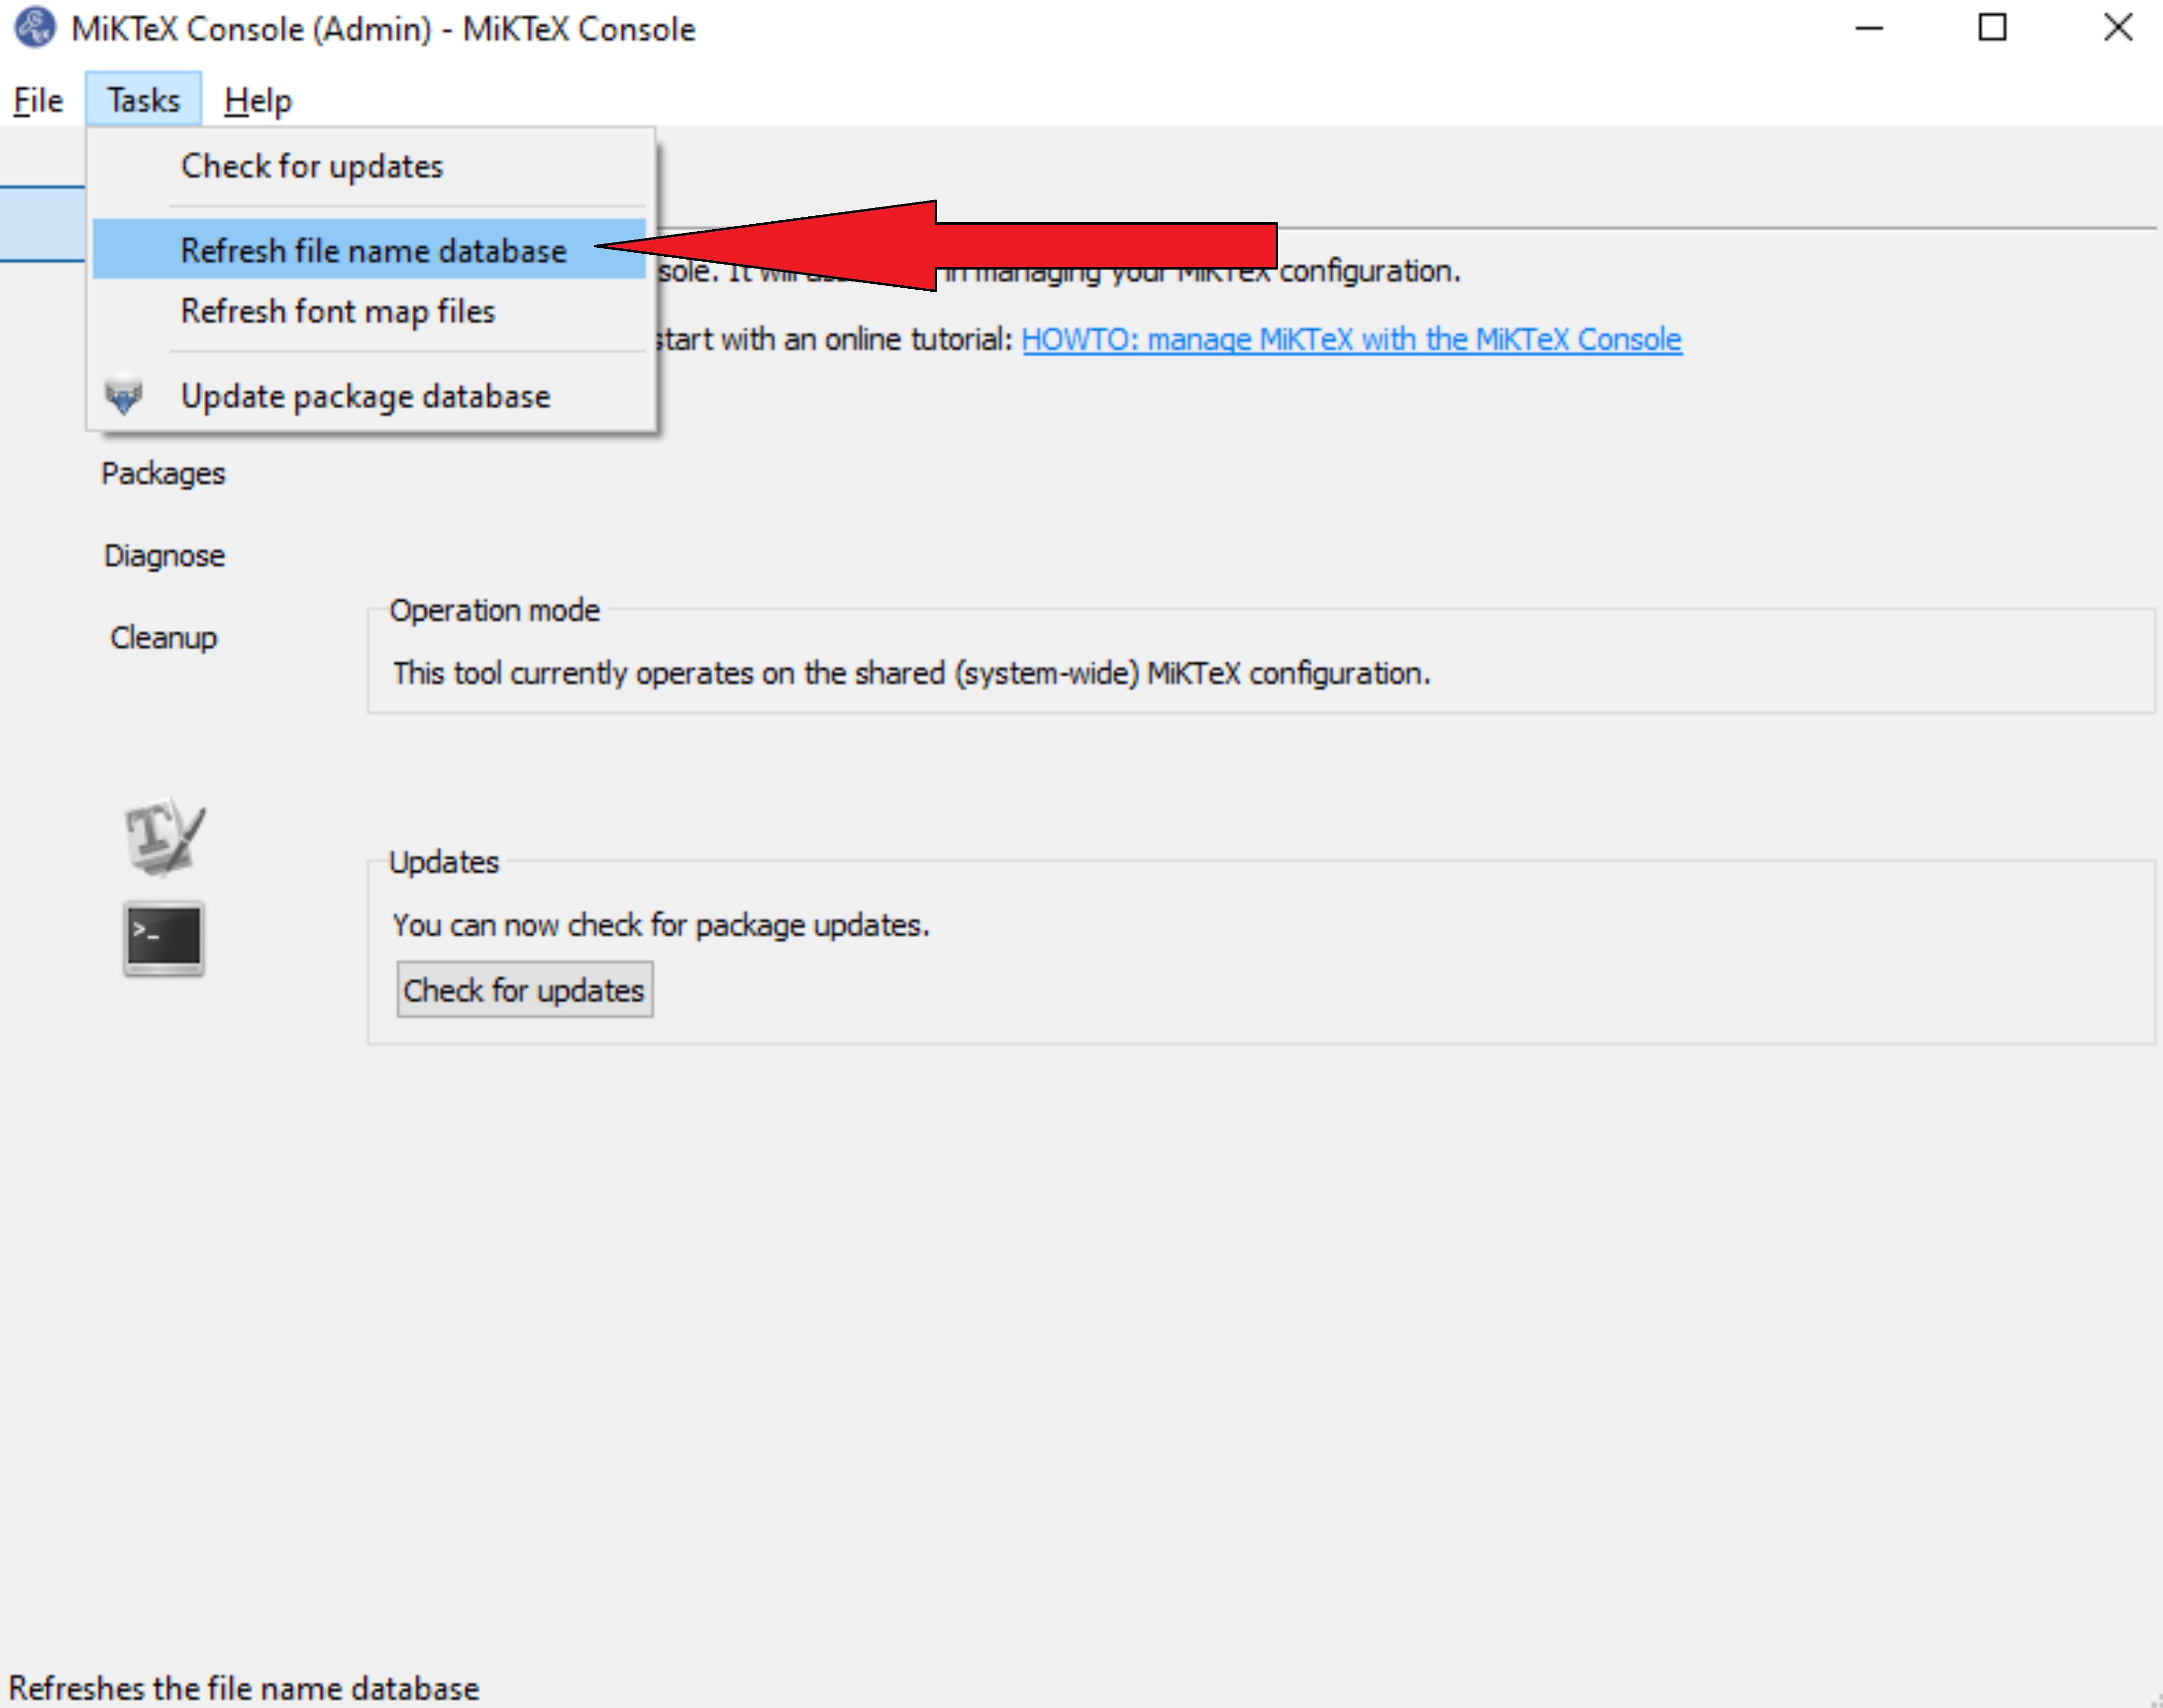
\includegraphics[width=0.9\textwidth]{MiKTeX}
  \label{fig:MiKTeX}
\end{figure}
%
%------------------------------------------------------------------------------
\subsection{Algumas dicas\ldots} 
%------------------------------------------------------------------------------
%
Toda vez que o \texttt{pdf} é construído, ou seja, toda vez que você realiza a
compilação do arquivo \texttt{.tex} principal, alguns arquivos são gerados, tais
como: \texttt{.aux}, \texttt{.log}, \texttt{.out} ou \texttt{.toc}.

Uma forma de organizar esses arquivos auxiliares é criar uma pasta e 
encaminha-los para lá.
Obviamente, isso pode ser feito manualmente, mas existem formas de automatização.
Para isso, você deve analisar a documentação do seu editor de texto para \LaTeX.
Mas, de uma forma geral, o comando utilizado é 
\begin{center}
 \texttt{-aux-directory=aux-files},
\end{center}
onde ``aux-files'' é o nome que aparecerá na pasta (pode ser escolhido outro 
nome, apenas evite acentos ou espaços no mesmo.). 

Pesquise como tal comando pode ser inserido no seu editor.

Para quem utiliza, por exemplo, o 
\href{https://www.texniccenter.org/}{\TeX~nicCenter}, o procedimento fica assim:
\marginpar{\qrcode[height = 1cm]{https://www.texniccenter.org/}}

No \TeX~nicCenter, siga o caminho: 
$\text{Build} \longrightarrow \text{Define Output Profiles}$. 
Aparecerá uma tela como a Figura~\ref{fig:aux-files}.

\begin{figure}[!htb]
 \centering
 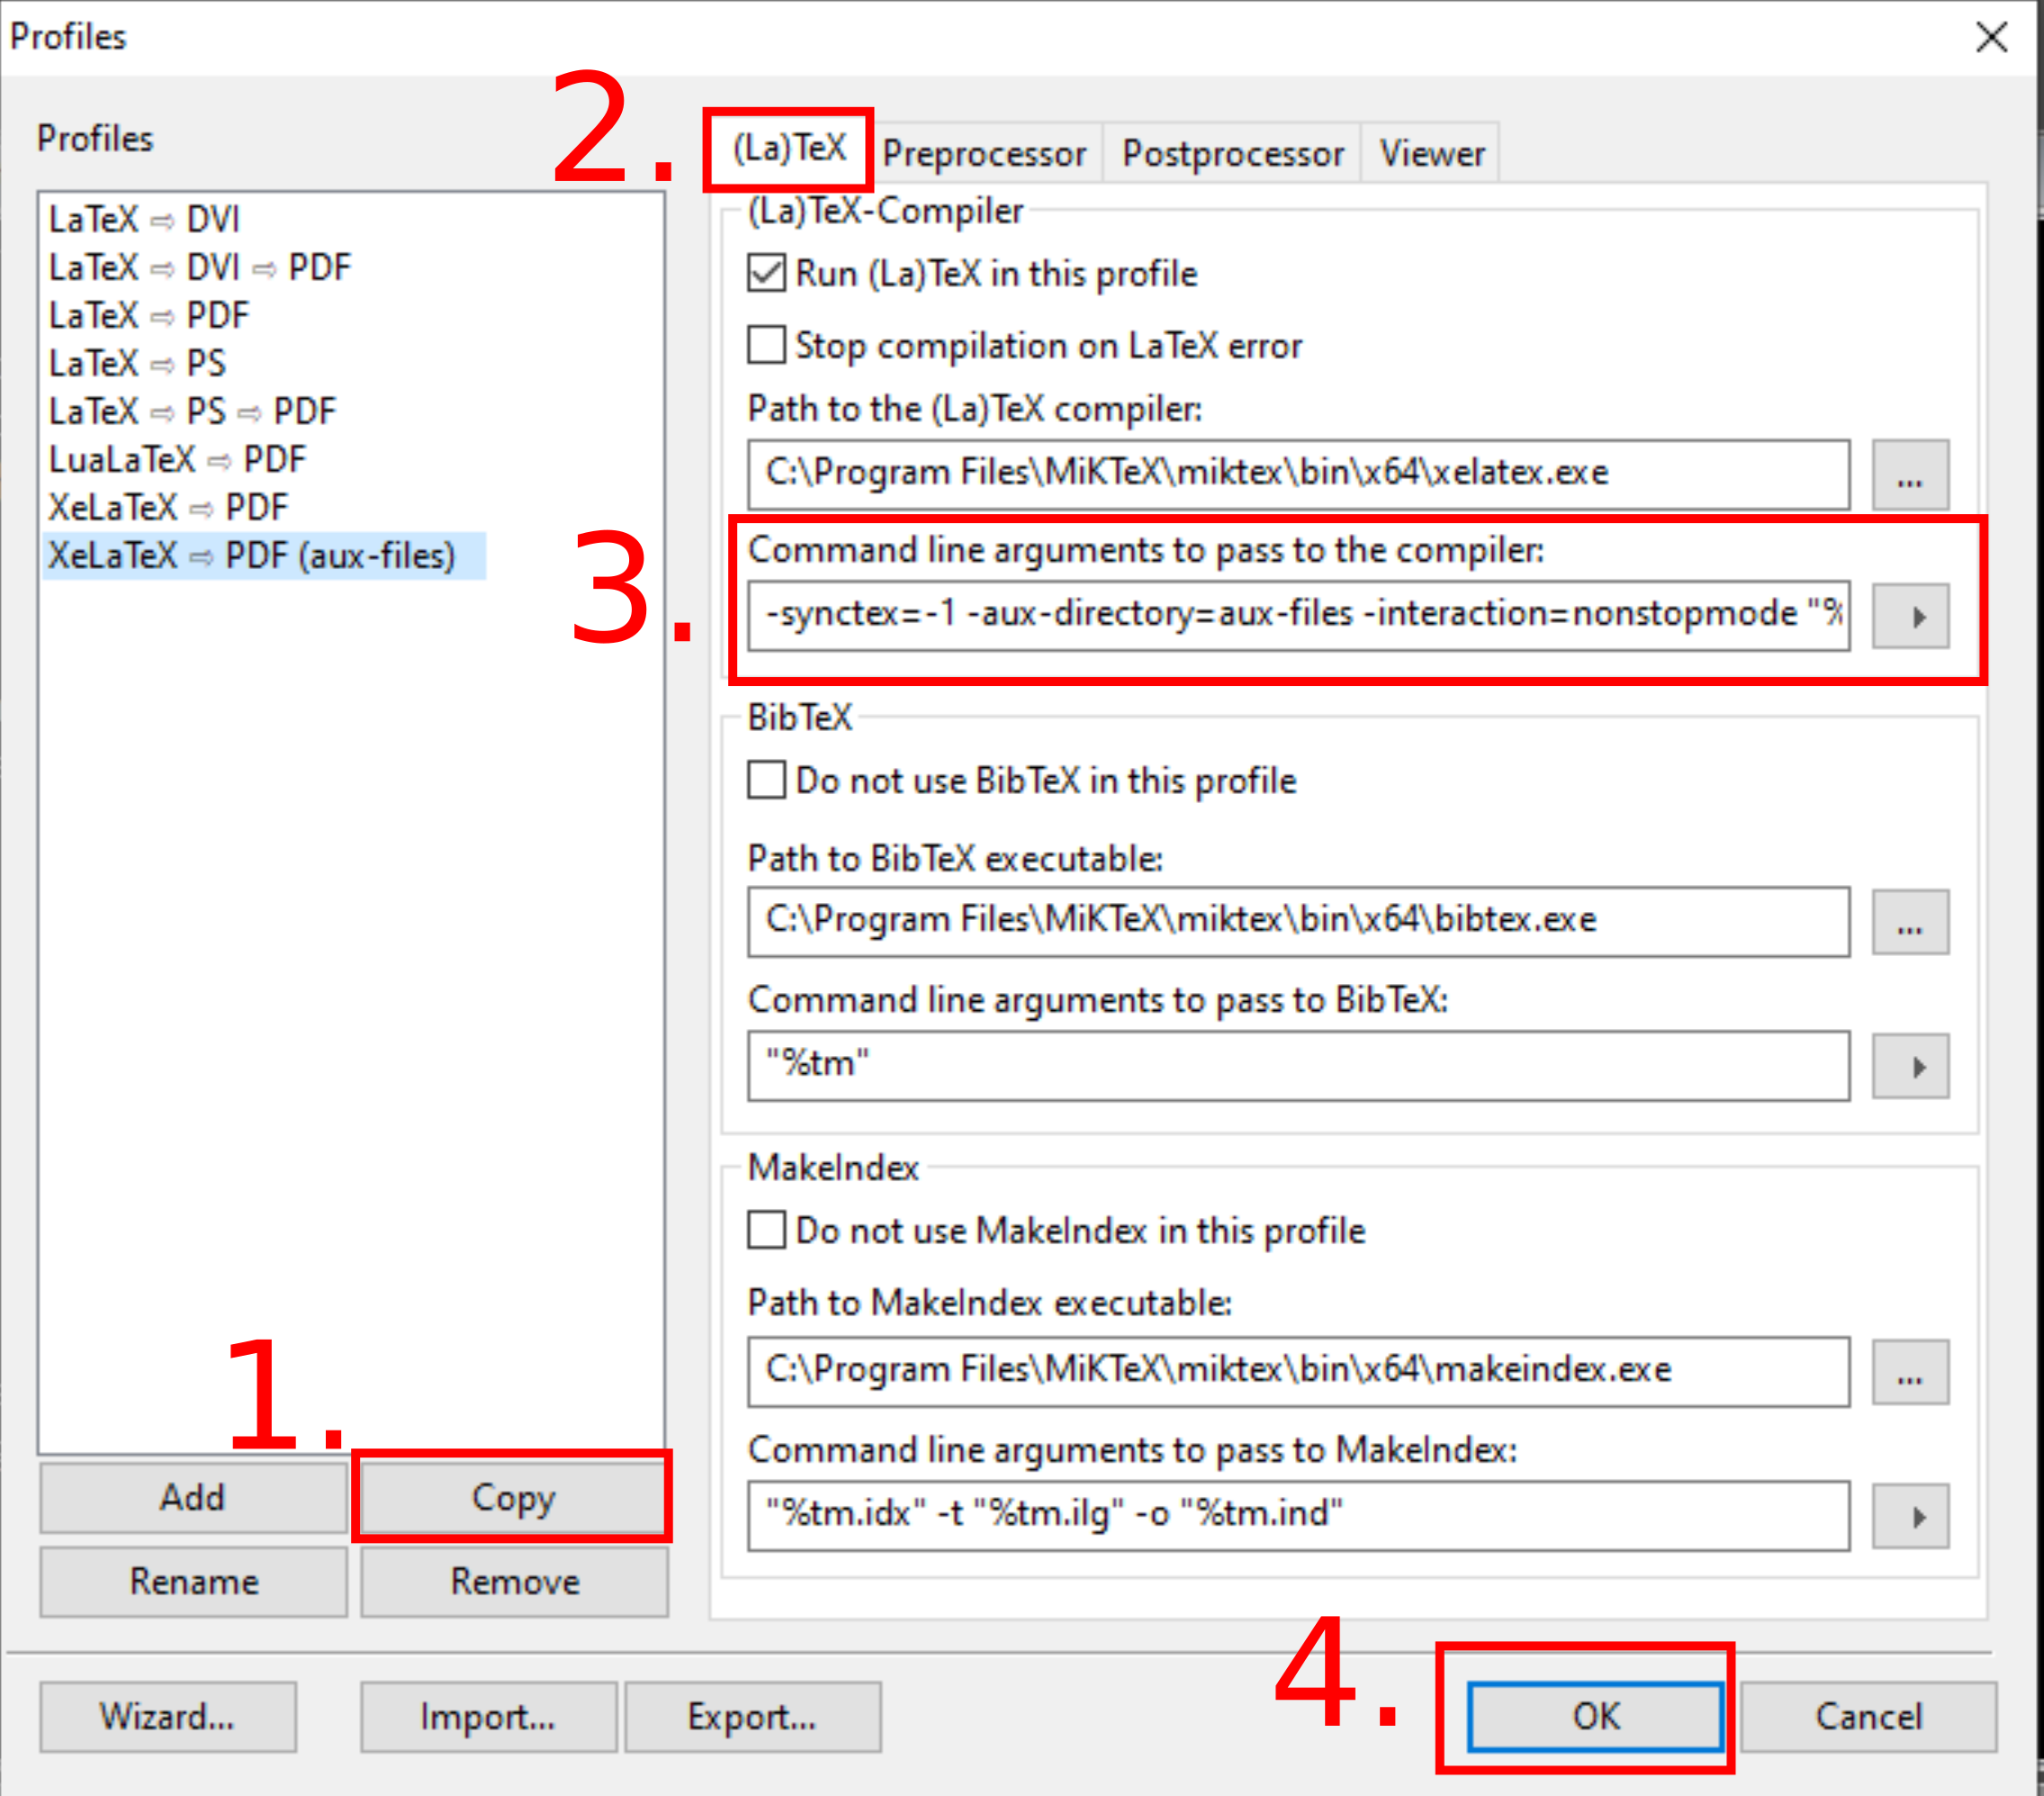
\includegraphics[width=0.9\textwidth]{aux-files}%
 \caption{Criando uma pasta para os arquivos auxiliares}%
 \label{fig:aux-files}%
\end{figure}

\begin{enumerate}
	\item Depois de escolher o compilador de sua preferência (no exemplo foi 
  escolhido o Xe~\LaTeX), clique no botão \textit{Copy} e faça uma cópia das 
  configurações do mesmo.
  Aparecerá uma caixa de texto para que você dê um nome para as configurações 
  da cópia (no exemplo, foi escolhido o nome
  ``$ \text{XeLaTeX} \Rightarrow \text{PDF } \text{(aux-files)}$'');
 \item Depois disso, na aba (La)TeX, faça o próximo passo;
 \item Na aba \texttt{Command line arguments to pass to the compiler}, antes do
  símbolo "\%wm", digite \texttt{-aux-directory=aux-files};
 \item Por fim, salve as novas configurações clicando em ``OK''.
\end{enumerate}

Assim, toda vez que você compilar (lembre de selecionar o compilador modificado,
ou seja, ``$ \text{XeLaTeX} \Rightarrow \text{PDF } \text{(aux-files)}$''), uma 
pasta \texttt{aux-files} será criada e todos os arquivos auxiliares citados 
serão encaminhados de forma automática para ela.

Há, também, um outro arquivo gerado ao produzir o \texttt{pdf}.
Tal arquivo possui extensão \texttt{.synctex}.
Serve para acesso ao texto em \LaTeX\ ao clicar, duplamente, sobre algum ponto
do \texttt{pdf}.
Caso você não queira essa surpreendente funcionalidade, pode deletar o arquivo.
